\documentclass{article}
\usepackage{graphicx}
\usepackage[svgnames]{xcolor}
\usepackage{fancyhdr}
\usepackage{tikz}
\usepackage{lipsum}
\usepackage{ifthen}
\usepackage{pgfmath}
\usepackage{amsmath}
\usepackage{listings}
\lstset{
  language=Python,
  basicstyle=\ttfamily,
  keywordstyle=\color{blue},
  stringstyle=\color{purple},
  commentstyle=\color{gray},
  numbers=left,
  numberstyle=\tiny\color{gray},
  frame=single,
  breaklines=true,
  breakatwhitespace=true,
  showstringspaces=false,
  tabsize=2
}
\usepackage{booktabs}
\usepackage[margin=1in, headheight=30pt, bottom=1in]{geometry}
\usepackage{xeCJK}

\setCJKmainfont{SimSun}
\definecolor{ponyPink}{RGB}{226,87,168}
\definecolor{ponyPurple}{RGB}{119,105,165}

\usetikzlibrary{calc}

\pagestyle{fancy}
\fancyhf{}
\fancyhead[L]{\textcolor{ponyPurple}{\sffamily\bfseries My Little Pony Template}}
\renewcommand{\headrulewidth}{0pt}
\begin{document}
\begin{titlepage}
	\centering
	\vspace*{2cm}
	{\fontsize{40}{48}\selectfont \textcolor{ponyPink}{\sffamily\bfseries My Little Pony Template}}
	\vskip1cm
	{\Large by Your Name}
	\vfill
	\includegraphics[width=6cm]{my_little_pony_icon5}
	\vfill
	{\Large May 2023}
\end{titlepage}

\fancyfoot[C]{\thepage}
\fancyfoot[R]{%
  \begin{tikzpicture}[baseline={(0,-0.5)}]
    \node[anchor=base,inner sep=0pt] at (0,0) {\includegraphics[width=0.7cm]{pony1}};
    \node[anchor=base,inner sep=0pt] at (0.7cm,0) {\includegraphics[width=0.7cm]{pony2}};
    \node[anchor=base,inner sep=0pt] at (1.4cm,0) {\includegraphics[width=0.7cm]{pony3}};
    \node[anchor=base,inner sep=0pt] at (2.1cm,0) {\includegraphics[width=0.7cm]{pony4}};
    \node[anchor=base,inner sep=0pt] at (2.8cm,0) {\includegraphics[width=0.7cm]{pony5}};
    \node[anchor=base,inner sep=0pt] at (3.5cm,0) {\includegraphics[width=0.7cm]{pony6}};
  \end{tikzpicture}
}


\lipsum[1-3]

\section{Demo Image}
\lipsum[4]
\begin{figure}[h]
	\centering
	\includegraphics[width=8cm]{demo_image}
	\caption{Demo Image}
	\label{fig:demo-image}
\end{figure}

\section{Mathematical Formulas}
\lipsum[5]
\begin{align*}
	f(x) & = x^2 + 2x + 1         \\
	g(x) & = \frac{1}{\sqrt{x+1}}
\end{align*}

\section{Table}
\lipsum[6]
\begin{table}[h]
	\centering
	\begin{tabular}{ccc}
		\toprule
		\textbf{Column 1} & \textbf{Column 2} & \textbf{Column 3} \\
		\midrule
		Value 1           & Value 2           & Value 3           \\
		Value 4           & Value 5           & Value 6           \\
		\bottomrule
	\end{tabular}
	\caption{Demo Table}
	\label{tab:demo-table}
\end{table}

\section{Highlighted Python Code}
\lipsum[7]
\begin{lstlisting}[language=Python, caption=Python Code, label=lst:python-code]
def factorial(n):
    if n == 0:
        return 1
    else:
        return n * factorial(n-1)

num = 5
print("Factorial of", num, "is", factorial(num))
\end{lstlisting}
% \section{Highlighted Python Code}
% \lipsum[7]
% \begin{lstlisting}[caption=Python Code, label=lst:python-code]
% def factorial(n):
% if n == 0:
% return 1
% else:
% return n * factorial(n-1)

% num = 5
% print("Factorial", "of", num, "is", factorial(num))
% \end{lstlisting}

\section{Demo TikZ Picture}
\lipsum[8]
\begin{figure}[h]
	\centering
	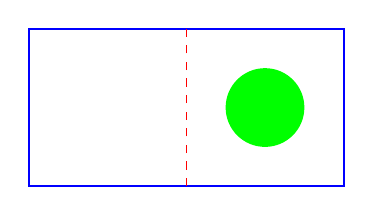
\begin{tikzpicture}
		\draw[blue, thick] (0,0) rectangle (4,2);
		\draw[red, dashed] (2,0) -- (2,2);
		\fill[green] (3,1) circle (0.5);
	\end{tikzpicture}
	\caption{Demo TikZ Picture}
	\label{fig:demo-tikz}
\end{figure}
\section{Demo Chinese}
这是一个中文句子的示例。
我喜欢小马宝莉。
中文也可以很好地显示在 LaTeX 文档中。
《小马宝莉:友情就是魔法》(英语:My Little Pony: Friendship is Magic,台湾译《彩虹小马:友情就是魔法》)是一部基于孩之宝小马宝莉系列玩具与动画作品,
由萝伦·浮士德为孩之宝开发的儿童奇幻动画剧集,常被称之为小马宝莉第四代(“G4”)产品,
由美国有线电视频道The Hub(Discovery Family的前身)于2010年10月10日首播。
该剧起初由萝伦·浮士德担任创意总监与执行制作,她寻求突破小马宝莉系列早已存在的“女孩”本质,
并依循着孩之宝对于“教育与资讯”内涵与玩具系列市场的建议,创造出更深刻的角色与更大胆的设定。
浮士德已于第二季中引退,由监制导演杰森·蒂森接手第二季之后的执行制作。
\section{Random words}
\lipsum[9-40]
\end{document}
